% \documentclass{beamer}
%Information to be included in the title page:
%\title{Moufangové rovina a spinové grupy}
%\author{Dominik Stejskal}
% \institute{Overleaf}
%\date{1. 4. 2022}

% test change after setting up offline backup

\documentclass[9pt]{beamer}

\usepackage{times,color}
\usepackage[czech]{babel}
\usepackage[utf8]{inputenc}
\usepackage{amsmath}
\usepackage[cmtip,all]{xy}
\usepackage[T1]{fontenc}
\usepackage[normalem]{ulem}

\usepackage{mathtools}   % přidal jsem já...

\newcommand{\End}{\mathrm{End}}
\newcommand{\Aut}{\mathrm{Aut}}
\newcommand{\Herm}{\mathrm{Herm}}
\newcommand{\orth}{\mathrm{O}}
\newcommand{\specorth}{\mathrm{SO}}
\newcommand{\Pin}{\mathrm{Pin}}
\newcommand{\Spin}{\mathrm{Spin}}
\newcommand{\mouf}{\mathbb{OP}_{\R}^2}
\def\R{\mathbb R}
\def\N{\mathbb N}
\def\C{\mathbb C}
\def\K{\mathbb K}
\def\Oct{\mathbb O}
\def\M{\mathrm{M}}
\DeclareMathOperator{\tr}{Tr}
\newtheorem{proposition}{Proposition}
%\newtheorem{theorem}{Theorem}
%\newtheorem{lemma}{Lemma}
%\newtheorem*{example}{Example}
\mode<presentation>
{
  \usetheme{Warsaw}
  \title{On the power of algebraic group models}
  \author{Dominik Stejskal}
  \date{Supervisor: Mgr. Pavel Hubáček, Ph.D.\\ \, \\2 June 2025}
}

%%%%%%%%%%%%%%%%%%%%%%%%%%%%%%%%%%%%%%%%%%%%%%%%%%%%%%%%%%%%%%%%%%%%%%

\begin{document}

\frame{\titlepage}




\begin{frame}
\frametitle{Overview}
\begin{itemize}
\item What are the important things about the thesis
\item etc.
\end{itemize}
\end{frame}


\begin{frame}
\frametitle{The end}
Thank you for your attention.
\end{frame}


\begin{frame}
\frametitle{Test slide}
\begin{itemize}
\item Item 1
\item Item 2
\end{itemize}
Free text.
\begin{align*}
1 + 1 &= 2 \\
2 + 2 &= 4
\end{align*}
\begin{theorem}[Name of the theorem]
$ 1+1=2. $
\end{theorem}
\end{frame}


\begin{frame}
\frametitle{Test slide with figure}
\centering
    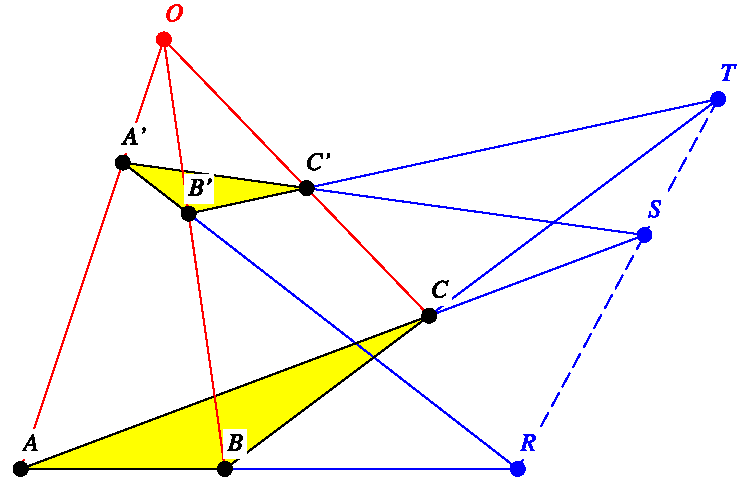
\includegraphics[width=10cm]{Desargues.pdf}
\end{frame}


\end{document}